% !TeX spellcheck = cs_CZ

\documentclass[a4paper]{article}
\usepackage[english]{babel}
\usepackage[utf8x]{inputenc}
\usepackage[T1]{fontenc}
\usepackage{listings}
\usepackage[a4paper,margin=2cm]{geometry}
\usepackage{amsmath}
\usepackage{graphicx}
\usepackage[colorlinks=true, allcolors=blue]{hyperref}
\usepackage{wasysym} % smileys
\usepackage{fancyhdr}
\usepackage{tikz}
\setlength\parindent{0pt} % indent

% my commands:
\newcommand{\n}{\newline}
\newcommand{\tab}{\hspace{1cm}}

\begin{document}

\thispagestyle{fancy} % beware the difference between \thispagestyle and \pagestyle
\lhead{5th homework, 05-11-2019}
\rhead{Vilém Zouhar}


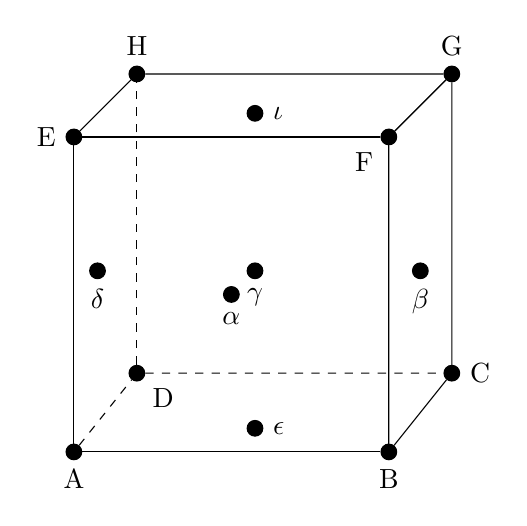
\begin{tikzpicture}
\foreach \n/\x/\l/\p in{
1/{( 0  , 0)}/{A}/below,
2/{( 4, 0)}/{B}/below,
3/{( .8, 1)}/{D}/south east,
4/{( 4.8, 1)}/{C}/right,
5/{( 0, 4)}/{E}/left,
6/{( 4, 4)}/{F}/south west,
7/{( 0.8, 4.8)}/{H}/above,
8/{( 4.8, 4.8)}/{G}/above,
9/{( 2, 2)}/{$\alpha$}/below,
9/{( 2.3, 2.3)}/{$\gamma$}/below,
9/{( 4.4, 2.3)}/{$\beta$}/below,
9/{( 0.3, 2.3)}/{$\delta$}/below,
9/{( 2.3, 4.3)}/{$\iota$}/right,
9/{( 2.3, 0.3)}/{$\epsilon$}/right
}
{
        \node[inner sep=2pt,circle,draw,fill,label={\p:\l}] (\n) at \x {};
    }
\draw[solid] (1) -- (2) -- (6) -- (5) -- (1);
\draw[solid] (5) -- (6) -- (8) -- (7) -- (5);
\draw[solid] (2) -- (4) -- (8) -- (6) -- (2);
\draw[dashed] (1) -- (3) -- (4);
\draw[dashed] (3) -- (7);
\end{tikzpicture}

\begin{tabular}{| l | l | l | l | p{35mm} |}
    \hline
    Rotation & $S_4$ type & $A_6$ type/example & $A_8$ type/example & $A_{12}$ type/example \\
    \hline 
    Identity & (4,0,0,0) & (6, 0, 0,0,0) & (8, 0, $\ldots$) & (12, 0, $\ldots$) \\
    \hline
    & & id & id & id \\
    \hline
   	Along the $x,y,z$ axes 90°& (0, 0, 0, 1) & (2,0,0,1,0,0) & (0, 0, 0, 2, $\ldots$) & (0, 0, 0, 3, $\ldots$)  \\
    \hline
    & & $(\epsilon, \beta, \iota, \delta)$ & $(ABFE)(CGHD)$ & $([EF][AE][BA][FB])$ $([CG][GH][HD][DC])$ $([GF][HE][DA][CB])$\\
    \hline
   	Along the $x,y,z$ axes 180°& (0, 2, 0, 0) & (2,2,0,0,0,0) & (0, 4, 0, $\ldots$) & (0, 6, 0, $\ldots$)  \\
    \hline
    & & $(\iota\epsilon)(\beta\delta)$ & $(AF)(EB)(DG)(HC)$ & $([HE][CB])([AD][FG])$ $([EF][AB])([EA][FB])$ $([CG][HD])([GH][CD])$ \\
   	\hline
   	Centers of opposite edges 180° & (2, 1, 0, 0) & (0,3,0,0,0,0) & (0, 4, 0, $\ldots$) & (2, 5, 0, $\ldots$)  \\
    \hline
    & & $(\alpha\epsilon)(\delta\beta)(\iota\gamma) $ & $(AB)(GH)(EC)(FD)$ & $([GF][DA])([HE][CB])$ $([CD][EF])([HD][GC])$ $([EA][FB])$\\
   	\hline
   	Opposing verticies & (1, 0, 1, 0) & (0,0,2,0,0,0) & (2, 3, 0, $\ldots$) & (0, 0, 4, $\ldots$)  \\
    \hline
    & & $(\alpha\delta\epsilon)(\iota\gamma\beta)$ & $(FD)(HB)(EC)$ & $([AB][AE][AD])$ $([HG][GC][GF])$ $([EF][HD][CB])$ $([FB][EH][CD])$\\
   	\hline
%  	Along the $x$ axis & & ($\iota$ $\gamma$, $\epsilon$ $\beta$) & ([HG][DC][AB][EF])& (EHDA)(FGCB) \\
%   	\hline
%   	Along the $y$ axis & & ($\iota$ $\beta$, $\epsilon$ $\delta$) & ([EH][FG][BC][AD])& (HGCD)(EFBA) \\
%   	\hline
%   	Along mid(AD) mid(FG) & & ($\alpha$ $\gamma$)($\iota$ $\beta$)($\delta$ $\epsilon$) & ([EH][FG][BC][AD])& (HGCD)(EFBA) \\
%   	\hline
   	
\end{tabular}

\end{document}
